\section{Resultados}

\subsection{Desempeño local}

La Tabla~\ref{tab:resultados-locales} resume cinco repeticiones medidas después de un calentamiento. Todas produjeron el hash \texttt{4eac656015050f40}.

\begin{table}[ht]
\centering
\caption{Escalabilidad fuerte local para una iteración base}
\label{tab:resultados-locales}
\begin{tabular}{rrrrr}
\toprule
MPI & OMP & $T$ (s) & $S_p$ & $E_p$ \\
\midrule
-- & -- & 3,672 & 1,000 & 1,000 \\
1 & 1 & 3,706 & 0,991 & 0,991 \\
1 & 2 & 1,870 & 1,964 & 0,982 \\
1 & 4 & 1,890 & 1,943 & 0,486 \\
2 & 2 & 1,876 & 1,957 & 0,489 \\
2 & 4 & 1,091 & 3,366 & 0,421 \\
\bottomrule
\end{tabular}
\end{table}

\begin{figure}[ht]
\centering
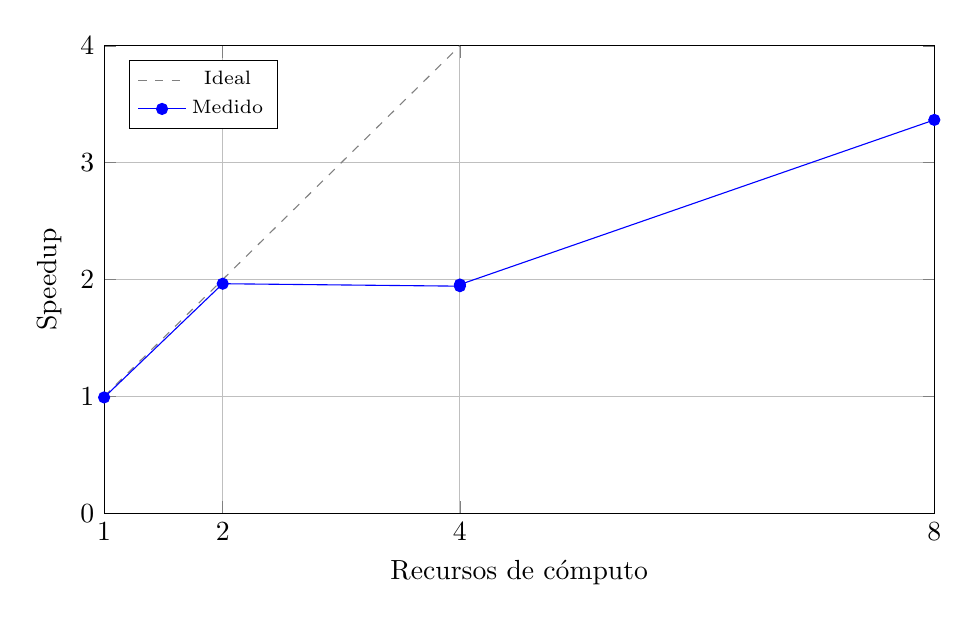
\begin{tikzpicture}
\begin{axis}[
    width=\columnwidth,
    height=0.62\columnwidth,
    xlabel={Recursos de cómputo},
    ylabel={Speedup},
    xmin=1,xmax=8,
    ymin=0,ymax=4,
    xtick={1,2,4,8},
    grid=major,
    legend style={font=\scriptsize,at={(0.03,0.97)},anchor=north west}
]
\addplot[dashed,gray] coordinates {(1,1) (2,2) (4,4)};
\addlegendentry{Ideal}
\addplot[mark=*,blue] coordinates {(1,0.991) (2,1.964) (4,1.943) (4,1.957) (8,3.366)};
\addlegendentry{Medido}
\end{axis}
\end{tikzpicture}
\caption{Speedup local respecto a la versión secuencial. Los dos puntos de cuatro recursos corresponden a $1\times4$ y $2\times2$.}
\label{fig:speedup-local}
\end{figure}

\subsubsection{Versión secuencial}

La mediana secuencial fue 3,672~s. La muestra máxima alcanzó 5,979~s, mientras las otras cuatro quedaron entre 3,631 y 3,740~s; por ello se usa la mediana como estadístico principal.

\subsubsection{Versión híbrida}

El costo del ejecutable híbrido con un recurso fue 0,9~\% mayor que el secuencial. Dos threads alcanzaron un speedup de 1,964, pero cuatro threads dentro de un solo proceso no mejoraron ese valor. La configuración $2\times4$ obtuvo el menor tiempo, 1,091~s, y un speedup de 3,366. En ella la búsqueda consumió 0,906~s, la preparación 0,057~s, los índices 0,086~s, la comunicación 0,041~s y la consolidación 0,019~s.

Con dos procesos el desbalance medio de trabajo fue 1,002, consistente con la distribución sintética casi uniforme. Se contabilizaron 4373 solicitudes remotas y 23,2~MB lógicos comunicados durante la iteración.

Una pasada adicional de los 120 meses mostró un comportamiento diferente. La versión secuencial demoró entre 32 y 36~s. La configuración $2\times4$ demoró entre 19,8 y 26,0~s; su mejor speedup observado fue 1,63. Esta comparación tiene una sola muestra por configuración y se usa para estimar la duración, no como resultado final. La menor mejora se explica porque, una vez que dejan de existir destinos válidos, las fases comunes y la comunicación tienen mayor peso que la búsqueda paralela.

\subsection{Desempeño en FING}

La Tabla~\ref{tab:resultados-fing} muestra las medianas de cinco repeticiones
del escenario completo de 120 meses. Todas las muestras produjeron el hash
\texttt{9de3a86b1efdd900}, igual al de la versión secuencial.

\begin{table}[ht]
\centering
\caption{Escalabilidad fuerte en FING para 120 meses}
\label{tab:resultados-fing}
\begin{tabular}{rrrrrr}
\toprule
MPI & OMP & $T$ (s) & $S_p$ & $E_p$ & Comunicación \\
\midrule
-- & -- & 28,584 & 1,000 & 1,000 & -- \\
1 & 1 & 32,141 & 0,889 & 0,889 & 0 \\
1 & 2 & 22,636 & 1,263 & 0,631 & 0 \\
1 & 4 & 20,623 & 1,386 & 0,347 & 0 \\
2 & 1 & 35,551 & 0,804 & 0,402 & 2,79 GB \\
2 & 2 & 34,758 & 0,822 & 0,206 & 2,79 GB \\
2 & 4 & 32,884 & 0,869 & 0,109 & 2,79 GB \\
\bottomrule
\end{tabular}
\end{table}

\begin{figure}[ht]
\centering
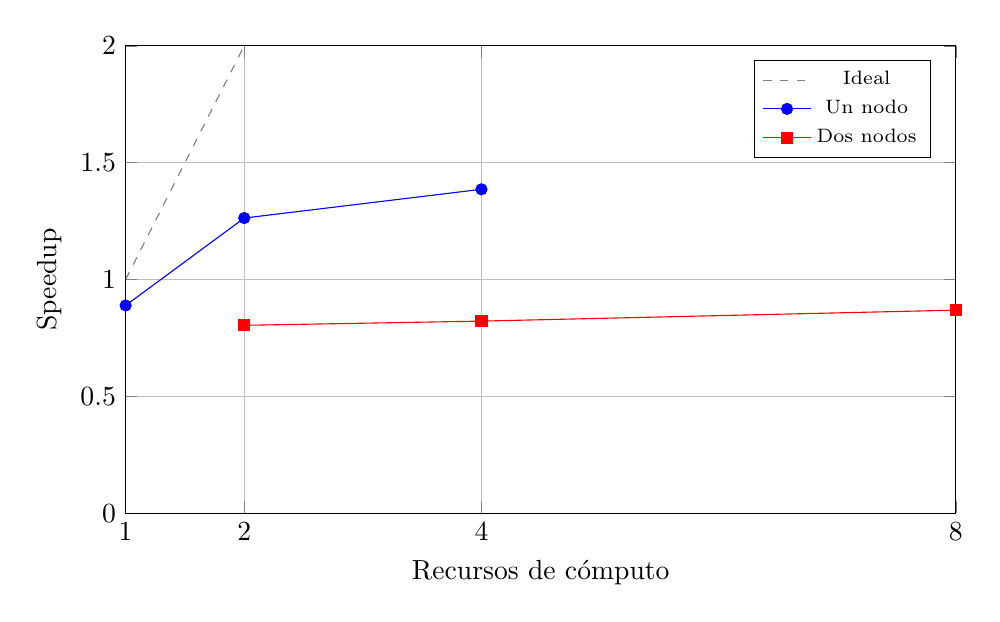
\begin{tikzpicture}
\begin{axis}[
    width=\columnwidth,
    height=0.62\columnwidth,
    xlabel={Recursos de cómputo},
    ylabel={Speedup},
    xmin=1,xmax=8,
    ymin=0,ymax=2,
    xtick={1,2,4,8},
    grid=major,
    legend style={font=\scriptsize,at={(0.97,0.97)},anchor=north east}
]
\addplot[dashed,gray] coordinates {(1,1) (2,2)};
\addlegendentry{Ideal}
\addplot[mark=*,blue] coordinates {(1,0.889) (2,1.263) (4,1.386)};
\addlegendentry{Un nodo}
\addplot[mark=square*,red] coordinates {(2,0.804) (4,0.822) (8,0.869)};
\addlegendentry{Dos nodos}
\end{axis}
\end{tikzpicture}
\caption{Speedup en FING respecto a la versión secuencial.}
\label{fig:speedup-fing}
\end{figure}

El menor tiempo fue 20,623~s con un proceso y cuatro hilos, un speedup de
1,386. Dos hilos, que corresponden a los dos núcleos físicos del equipo,
alcanzaron 22,636~s. Los cuatro hilos aprovecharon además los hilos lógicos del
procesador, pero la mejora adicional fue menor.

Las configuraciones de dos procesos fueron más lentas que la secuencial. En
los 120 meses intercambiaron 2,79~GB lógicos y atendieron 195391 solicitudes
remotas. El desbalance medio fue solamente 1,005, por lo que la diferencia no
se explica por una mala división del trabajo. El costo proviene principalmente
del intercambio y de mantener datos globales en ambos procesos.

\subsection{Comportamiento del modelo}

En la primera iteración base, 291147 de 522351 hogares estaban satisfechos (55,7~\%). Se generaron 222341 solicitudes, de las cuales 28258 fueron aceptadas y 194083 rechazadas por conflicto; otros 8863 hogares insatisfechos no hallaron destino viable. En el mes 14 se alcanzaron 333477 hogares satisfechos (63,8~\%) y no se produjo ninguna nueva solicitud. Desde ese punto hasta el mes 120, 188874 hogares permanecieron insatisfechos porque ninguna vivienda vacía cumplía a la vez sus preferencias y su capacidad de pago. Las viviendas se liberaron correctamente; el estado quedó trabado por las reglas del escenario sintético.

\subsection{Sensibilidad}

En el escenario mediano se compararon diez iteraciones base, sin ruido de precios y sin permanencia mínima. Los hogares satisfechos finales fueron 20955, 20941 y 20966, respectivamente, sobre 32691 hogares: una variación menor a 0,1 puntos porcentuales. Sin permanencia no quedaron hogares bloqueados, como exige la definición. Las solicitudes y hogares sin destino variaron ampliamente entre escenarios en la décima iteración, indicando que una observación mensual aislada no caracteriza la dinámica; el análisis final deberá usar series completas y varias semillas.
